
% wissdoc Optionen: draft, relaxed, pdf, oneside --> siehe wissdoc.cls
%\documentclass{wissdoc}
\documentclass[oneside]{wissdoc}


% Packages für Deckblatt (u.a.)
\usepackage[absolute]{textpos} 	%Textboxen an absolute Position setzen
\usepackage{setspace}						%Zeilenabstand anpassen
%\usepackage{color}							%Farbige Schrift
\usepackage[dvipsnames,table,xcdraw]{xcolor}
\usepackage{graphicx}						%Einbinden von Grafiken
\usepackage{subfigure}
\usepackage{caption}
\usepackage{rotating}
\usepackage{lscape}
\usepackage{multirow}


% language / input
\usepackage[ngerman]{babel}
\usepackage[T1]{fontenc}
\usepackage[utf8]{inputenc}


% listings for code
\usepackage{listings}
\newcommand\YAMLcolonstyle{\color{red}\mdseries}
\newcommand\YAMLkeystyle{\color{black}\bfseries}
\newcommand\YAMLvaluestyle{\color{blue}\mdseries}
\lstset{basicstyle=\ttfamily} % fixed-width font
\lstset{tabsize=4}

% also minted for code
\usepackage{minted}


% glossaries
\usepackage{url}
\usepackage[acronym,toc]{glossaries}

\makeglossaries

\usepackage{xparse}
\DeclareDocumentCommand{\newdualentry}{ O{} O{} m m m m } {
  \newglossaryentry{gls-#3}{name={#4},text={#4\glsadd{#3}},
    description={#6},#1
  }
  \makeglossaries
  \newacronym[see={[Glossary:]{gls-#3}},#2]{#3}{#4}{#5\glsadd{gls-#3}}
}

\loadglsentries{glossaries}


% bib stuff
\usepackage[autostyle]{csquotes}

\usepackage[
    backend=biber,
    style=ieee,
    sortlocale=de_DE,
    natbib=true,
    url=true,
    doi=true,
    eprint=false
]{biblatex}
\addbibresource{literatur.bib}

\usepackage[]{hyperref}
\hypersetup{
    colorlinks=false,
    linkbordercolor=gray,
    urlbordercolor=blue
    %urlcolor=blue,
    %linkcolor=black
}

% license
\usepackage[
    type={CC},
    modifier={by-sa},
    version={3.0},
]{doclicense}


%\usepackage[footnote]{acronym}

% Zeilenabstand nach Vorgabe - Falls gefordert
%\setstretch{1,3} 

% Inhaltsangabe auf Unterabschnitte(2 Ebenen) begrenzen
\setcounter{tocdepth}{2}


% \usepackage{color}    % Farbiger/grauer Text
% \usepackage{colortbl}   % Farbige/graue Tabellenzeilen und -spalten!! <--
% \usepackage{fancybox} % für schattierte,ovale Boxen etc.
% \usepackage{tabularx} % automatische Spaltenbreite
% \usepackage{supertab} % mehrseitige Tabellen
%% ---------------- end of usepackages -------------

%% Informationen für die PDF-Datei
\hypersetup{pdfauthor={Domenik Müller},%
            pdftitle={Bachelorarbeit: FPGA-Event-Recorder},%
            pdfsubject={Design und Implementierung eines FPGA-Event-Recorders mit der freien IceStorm-Toolchain},%
            pdfkeywords={FPGA, Open Source, IceStorm, iCE40, Lattice},%
            pdfproducer={LaTeX},%
            pdfcreator={pdfLaTeX}
}

% Macros, nicht unbedingt notwendig
%%%%%%%%%%%%%%%%%%%%%%%%%%%%%%%%%%%%%%%%%%%%%%%%%%%%%%%%%%
% macros.tex -- einige mehr oder weniger nuetzliche Makros
%%%%%%%%%%%%%%%%%%%%%%%%%%%%%%%%%%%%%%%%%%%%%%%%%%%%%%%%%%


%%%%%%%%%%%%%%%%%%%%%%%
% Kommentare 
%%%%%%%%%%%%%%%%%%%%%%%
\ifnotdraftelse{
\newcommand{\Kommentar}[1]{}
}{\newcommand{\Kommentar}[1]{{\em #1}}}
% Alles innerhalb von \Hide{} oder \ignore{} 
% wird von LaTeX komplett ignoriert (wie ein Kommentar)
\newcommand{\Hide}[1]{}
\let\ignore\Hide

%%%%%%%%%%%%%%%%%%%%%%%%%
% Leere Seite ohne Seitennummer, wird aber gezaehlt
%%%%%%%%%%%%%%%%%%%%%%%%%

\newcommand{\leereseite}{% Leerseite ohne Seitennummer, n�chste Seite rechts (wenn 2-seitig)
 \clearpage{\pagestyle{empty}\cleardoublepage}
}

%%%%%%%%%%%%%%%%%%%%%%%%%%
% Neue Seite rechts, leere linke Seite ohne Headings
%%%%%%%%%%%%%%%%%%%%%%%%%%
\newcommand{\xcleardoublepage}
{{\pagestyle{empty}\cleardoublepage}}

%%%%%%%%%%%%%%%%%%%%%%%%%%
% Tabellenspaltentypen (benoetigt colortbl)
%%%%%%%%%%%%%%%%%%%%%%%%%%
\newcommand{\PBS}[1]{\let\temp=\\#1\let\\=\temp}
\newcolumntype{y}{>{\PBS{\raggedright\hspace{0pt}}}p{1.35cm}}
\newcolumntype{z}{>{\PBS{\raggedright\hspace{0pt}}}p{2.5cm}}
\newcolumntype{q}{>{\PBS{\raggedright\hspace{0pt}}}p{6.5cm}}
\newcolumntype{g}{>{\columncolor[gray]{0.8}}c} % Grau
\newcolumntype{G}{>{\columncolor[gray]{0.9}}c} % helleres Grau

%%%%%%%%%%%%%%%%%%%%%%%%%%
% Anf�hrungszeichen oben und unten
%%%%%%%%%%%%%%%%%%%%%%%%%%
\newcommand{\anf}[1]{"`{#1}"'}

%%%%%%%%%%%%%%%%%%%%%%%%%%
% Tiefstellen von Text
%%%%%%%%%%%%%%%%%%%%%%%%%%
% S\tl{0} setzt die 0 unter das S (ohne Mathemodus!)
% zum Hochstellen gibt es uebrigens \textsuperscript
\makeatletter
\DeclareRobustCommand*\textlowerscript[1]{%
  \@textlowerscript{\selectfont#1}}
\def\@textlowerscript#1{%
  {\m@th\ensuremath{_{\mbox{\fontsize\sf@size\z@#1}}}}}
\let\tl\textlowerscript
\let\ts\textsuperscript
\makeatother

%%%%%%%%%%%%%%%%%%%%%%%%%%
% Gau�-Klammern
%%%%%%%%%%%%%%%%%%%%%%%%%%
\newcommand{\ceil}[1]{\lceil{#1}\rceil}
\newcommand{\floor}[1]{\lfloor{#1}\rfloor}

%%%%%%%%%%%%%%%%%%%%%%%%%%
% Average Operator (analog zu min, max)
%%%%%%%%%%%%%%%%%%%%%%%%%%
\def\avg{\mathop{\mathgroup\symoperators avg}}

%%%%%%%%%%%%%%%%%%%%%%%%%%
% Wortabk�rzungen
%%%%%%%%%%%%%%%%%%%%%%%%%%
\def\zB{z.\,B.\ }
\def\dh{d.\,h.\ }
\def\ua{u.\,a.\ }
\def\su{s.\,u.\ }
\newcommand{\bzw}{bzw.\ }

%%%%%%%%%%%%%%%%%%%%%%%%%%%%%%%%%%%
% Einbinden von Graphiken
%%%%%%%%%%%%%%%%%%%%%%%%%%%%%%%%%%%
% global scaling factor
\def\gsf{0.9}
%% Graphik, 
%% 3 Argumente: Datei, Label, Unterschrift
\newcommand{\Abbildung}[3]{%
\begin{figure}[tbh] %
\centerline{\scalebox{\gsf}{\includegraphics*{#1}}} %
\caption{#3} %
\label{#2} %
\end{figure} %
}
\let\Abb\Abbildung
%% Abbps
%% Graphik, skaliert, Angabe der Position
%% 5 Argumente: Position, Breite (0 bis 1.0), Datei, Label, Unterschrift
\newcommand{\Abbildungps}[5]{%
\begin{figure}[#1]%
\begin{center}
\scalebox{\gsf}{\includegraphics*[width=#2\textwidth]{#3}}%
\caption{#5}%
\label{#4}%
\end{center}
\end{figure}%
}
\let\Abbps\Abbildungps
%% Graphik, Angabe der Position, frei w�hlbares Argument f�r includegraphics
%% 5 Argumente: Position, Optionen, Datei, Label, Unterschrift
\newcommand{\Abbildungpf}[5]{%
\begin{figure}[#1]%
\begin{center}
\scalebox{\gsf}{\includegraphics*[#2]{#3}}%
\caption{#5}%
\label{#4}%
\end{center}
\end{figure}%
}
\let\Abbpf\Abbildungpf

%%
% Anmerkung: \resizebox{x}{y}{box} skaliert die box auf Breite x und H�he y,
%            ist x oder y ein !, dann wird das uspr�ngliche 
%            Seitenverh�ltnis beibehalten.
%            \rescalebox funktioniert �hnlich, nur das dort ein Faktor
%            statt einer Dimension angegeben wird.
%%
% \Abbps{Position}{Breite in Bruchteilen der Textbreite}{Dateiname}{Label}{Bildunterschrift}
%

\newcommand{\refAbb}[1]{%
s.~Abbildung \ref{#1}}

%%%%%%%%%%%%%%%%%%%%
%% end of macros.tex
%%%%%%%%%%%%%%%%%%%%

% Print URLs not in Typewriter Font
\def\UrlFont{\rm}

\newcommand{\blankpage}{% Leerseite ohne Seitennummer, nächste Seite rechts
 \clearpage{\pagestyle{empty}\cleardoublepage}
}

%% Einstellungen für das gesamte Dokument

% Trennhilfen
% Wichtig!
% Im german-paket sind zusätzlich folgende Trennhinweise enthalten:
% "- = zusätzliche Trennstelle
% "| = Vermeidung von Ligaturen und mögliche Trennung (bsp: Schaf"|fell)
% "~ = Bindestrich an dem keine Trennung erlaubt ist (bsp: bergauf und "~ab)
% "= = Bindestrich bei dem Worte vor und dahinter getrennt werden dürfen
% "" = Trennstelle ohne Erzeugung eines Trennstrichs (bsp: und/""oder)

% Trennhinweise fuer Woerter hier beschreiben
\hyphenation{
% Pro-to-koll-in-stan-zen
% Ma-na-ge-ment  Netz-werk-ele-men-ten
% Netz-werk Netz-werk-re-ser-vie-rung
% Netz-werk-adap-ter Fein-ju-stier-ung
% Da-ten-strom-spe-zi-fi-ka-tion Pa-ket-rumpf
% Kon-troll-in-stanz
}

%Tabellen Kommandos
\newcolumntype{L}[1]{>{\raggedright\arraybackslash}p{#1}}
\newcolumntype{C}[1]{>{\centering\arraybackslash}p{#1}}
\newcolumntype{R}[1]{>{\raggedleft\arraybackslash}p{#1}}

% Index-Datei öffn
\makeindex



\begin{document}

\pagenumbering{gobble}

%%% Deckblatt - Hochschule Augsburg
%%%Deckblatt

\textblockorigin{20mm}{30mm}

\thispagestyle{empty}\null
%%%%Logo - Hochschule Augsburg - Informatik
\begin{textblock}{10}(8.0,1.1)
\begin{figure}[h]
	\centering
		
\includegraphics[width=0.45\textwidth]{logos/hsa_informatik_logo_lq.pdf}
\end{figure}

\end{textblock}

%%% Text unter Logo
\begin{textblock}{15}(12.43,2.1)
	\LARGE
	\textsf{
		\textbf{\textcolor[rgb]{1,0.41,0.13}{\\
			\begin{flushleft}
				Fakultät für\\
				Informatik\\
			\end{flushleft}
			}
		}
	}
\end{textblock}

%%%%Textbox links - Informationen
\begin{textblock}{15}(2,1.4)
	%\LARGE
	\begin{flushleft}
		\begin{spacing} {1.2}
			\LARGE	
				\vspace{150pt}
				\textcolor[rgb]{1,0.41,0.13}{\\
				\textbf{Bachelorarbeit}}\\
				\vspace{10pt}
			\LARGE   \textbf{Desgin und Implementierung \\eines FPGA-Event-Recorders mithilfe \\der freien IceStorm-Toolchain} \\			
			\Large
				\vspace{10pt}		
				Studienrichtung: Technische Informatik\\
				\vspace{30pt}
				Domenik Müller\\
				\vspace{110pt}		
				\vspace{80pt}		
			\Large
				Prüfer: Prof. Dr. Hubert Högl\\
				Zweitprüfer: Prof. Dr. Alexander von Bodisco\\ 
				\vspace{7pt}		
				Abgabedatum: 20.06.2018\\
			\end{spacing}
		\end{flushleft}
		
\end{textblock}



%%%%Textbox rechts - Hochschule
\begin{textblock}{5}(12.45,9.0)
	\scriptsize
	\textcolor[rgb]{1,0,0}{\\
		\begin{flushleft}
			\begin{spacing} {1.3}
				Hochschule f\"ur angewandte\\
				Wissenschaften Augsburg\\
				\vspace{4pt}
				An der Hochschule 1\\
				D-86161 Augsburg\\
				\vspace{4pt}
				Telefon +49 821 55 86-0\\
				Fax +49 821 55 86-3222\\
				www.hs-augsburg.de\\
				info@hs-augsburg.de
			\end{spacing}
		\end{flushleft}
		}
\end{textblock}


%%%%Textbox rechts unten - Fakultät und Autor
\begin{textblock}{5}(12.45,11.5)
	\scriptsize
		\begin{flushleft}
			\begin{spacing} {1.3}
				Fakult\"at f\"ur Informatik\\
				Telefon +49 821 55 86-3450\\
				Fax \hspace{10pt} +49 821 55 86-3499\\
				\vspace{6pt}
				Verfasser der Bachelorarbeit\\
				Domenik Müller\\
				Am Eser 3\\
				86150 Augsburg\\
				Telefon +49 821 44 92 57 54\\
				domenikmueller@gmx.net\\
			\end{spacing}
		\end{flushleft}
	\end{textblock}
\pagebreak
  %<-- Nach Vorgabe der HS Augsburg


%
%% ++++++++++++++++++++++++++++++++++++++++++
%% Verzeichnisse
%% ++++++++++++++++++++++++++++++++++++++++++

\section*{Zusammenfassung}

In der vorliegenden Arbeit wird der Entwurf und die Implementierung eines FPGA-basierten Event-Recorders mithilfe der Open-Source-Toolchain IceStorm beschrieben. Ähnlich wie bei einem Logikanalysator werden digitale Signale an den Eingängen erfasst, allerdings wird der Signalzustand an den Eingängen nicht wie bei einem Logikanalysator kontinuierlich übertragen, sondern es wird bereits zur Erfassungszeit nach relevanten Signaländerungen und Eingangskombinationen gefiltert. Eine Filterung nach benutzerdefinierten Events bietet sich vor allem für die Analyse von bekannten Signalen an, deren Ablauf mit möglichst hoher zeitlicher Auflösung abgebildet werden soll.
Die Implementierung des Event-Recorders erfolgt auf einem Raspberry Pi Zero mit einem Lattice iCE40-basierten FPGA-Shield und wird vollständig mit den von der IceStorm-Toolchain zur Verfügung gestellten Open-Source-Tools und Komponenten umgesetzt.   

\section*{Abstract}

The work in hand describes the design and implementation of a FPGA based event recorder using the open source toolchain IceStorm. 
Similar to a logic analyzer it records logic level input signals, but in contrast to a logic analyzer it does not provide a continuous stream of the input signal state. Instead the signals are filtered at capture time to match only relevant input combinations and signal changes. Using predefined events to filter the input stream is especially suitable for the analysis of known signals that are to be captured and examined at high temporal resolution.
The implementation of the event recorder is done on a Raspberry Pi Zero with a Lattice iCE40-based FPGA shield and is realized completely with the tools and components provided by the open source toolchain IceStorm.   


\ifnotdraft{
\tableofcontents
% Leere Seite bei zweiseitigem Druck
%\ifnotonesideelse{\blankpage}{}
%\listoffigures
%% Leere Seite bei zweiseitigem Druck
%\ifnotonesideelse{\blankpage}{}
%\listoftables
%% Leere Seite bei zweiseitigem Druck
%\ifnotonesideelse{\blankpage}{}
}

\clearpage


%% ++++++++++++++++++++++++++++++++++++++++++
%% Hauptteil
%% ++++++++++++++++++++++++++++++++++++++++++
\graphicspath{{figures/}}
\pagenumbering{arabic}


%%% Ab hier eigene Kapitel einfügen
%%% Kapitel sind analog zur Wordvorlage zu wählen
\chapter{Einführung}

\label{ch:Einfuehrung}

Mikrocontroller werden heute in Gebrauchsgegenständen aller Art verbaut und werden den Anforderungen entsprechend immer leistungsstärker und damit unter anderem auch schneller. Selbst einfache Mikrocontroller arbeiten oft mit einer Geschwindigkeit im mehrstelligen Megaherz Bereich (sprich: mehrere Millionen Takte pro Sekunde). Im Unterschied zu klassischen PC-Systemen werden an Mikrocontroller oft Echtzeit-Anforderungen gestellt, das heißt Ergebnisse müssen zuverlässig innerhalb einer vorbestimmten Zeitspanne geliefert werden\cite{wiki:echtzeit}. Dabei wird auch die Hardware von Mikrocontrollern zunehmend komplexer und es werden vermehrt Mehrprozessor-Systeme verwendet, die angepasste und mitunter unübersichtlichere Programmiertechniken erfordern.\\ 
Dementsprechend werden für die Entwicklung von Mikrocontroller-Systemen (aber auch von digitalen Systemen im allgemeinen) Werkzeuge benötigt, mit denen Signale mit hoher zeitlicher Auflösung erfasst und analysiert werden können.\\
Ergänzend zu Simulations- und Software-gestützten Verfahren wird diese Aufgabe meist von Logikanalysatoren erfüllt, die die an den Eingängen anliegenden Spannungen mit einer festen Frequenz erfassen und die Daten dann zum Beispiel an einen PC übertragen, an dem sie ausgewertet werden können.\\
In der vorliegenden Arbeit wird eine spezielle Form von Logikanalysator entworfen, bei der ein Teil der Auswertung bereits auf dem Logikanalysator durchgeführt wird. Das Eingangssignal wird auf bestimmte - vom Benutzer definierte - Signaländerungen untersucht und nur relevante Signaländerungen (``Events'') werden an den Benutzer weitergereicht.\\
Dieses Vorgehen bietet sich vor allem dann an, wenn der Signalverlauf grundsätzlich bekannt ist und der Fokus der Analyse auf den exakten zeitlichen Abbildung des erwarteten Signalverlaugs liegt.\\
Ein Beispiel wären die Ausgänge eines Mikrocontrollers, bei dem bewusst bestimmte Kombinationen gesetzt werden um den Start und das Ende von Funktionen im Quellcode zu signalisieren. Da das Setzen von GPIO-Pins meist in einem einzigen CPU-Takt ausgeführt werden kann, können so zuverlässige Aussagen zur Laufzeit von Funktionen, oder bei periodischer Ausführung auch zur zeitlichen Fluktuation der Funktionsausführung (``Jitter-Analyse'') getroffen werden.

\clearpage

\section{Zielsetzung}
\label{ch:Einfuehrung:Zielsetzung}

%Grundvoraussetzung für die Aufnahme aussagekräftiger Signaldaten ist die kontinuierliche Erfassung des Eingangssignals bei gleichbleibendem Zeitabstand. 
Für die Implementierung des Event-Recorders wurden folgende technische Ziele angestrebt:
\begin{itemize}
\item Es soll der logische Pegel von 8 bis 16 Eingangs-Pins abgefragt werden und die Eingangsdaten sollen mit einem stabilen Zeitstempel versehen werden.
\item Die zeitliche Auflösung der Aufnahme soll im Megaherz-Bereich liegen
\item Bestimmte Eingangskombinationen sollen in Textform definiert, und bei der Aufnahme als Events erkannt werden
\item Zur Steuerung der Aufnahme soll ein Kommandozeilentool zur Verfügung stehen, mit dem auch die aufgenommenen Daten in Textform abgespeichert werden können.
\end{itemize} 


\section{Motivation}
\label{ch:Einfuehrung:Motivation}

Die Arbeit schließt thematisch an die Bachelorarbeit ``Ein universales, rekonfigurierbares und freies USB-Gerät zur Timing-, Protokoll-, Logik- und Eventanalyse von digitalen Signalen'' von Andreas Müller und einer darauf folgenden Projektarbeit an.\\
In der Bachelorarbeit wurde eine Hardware-Platine namens ``USB-TPLE'' mit USB-Schnittstelle, einem \acrshort{CPLD}-Chip von Altera und einem Atmega Mikrocontroller für die selbe Zielsetzung entworfen, und mit der Software-Implementierung begonnen\cite{ba:mueller}.\\  
Im nachfolgenden Semester-Projekt ``Logikanalysator mit AVR Mega32U4 und Altera MAX CPLD'' im Wintersemester 2013/14 wurde die Software-Implementierung ausgebaut und eine funktionsfähige Konfiguration für den CPLD-Chip entwickelt.\\

Im folgenden wird allerdings ein anderer Ansatz für die Umsetzung verfolgt:
\begin{description}
\item[Verwendung von käuflich verfügbarer Hardware] \hfill \\
Anstatt der selbst entworfenen Platine soll aus Gründen der Vefügbarkeit und um die Einstiegshürde für Benutzer zu verringern ein käuflich erwerbbares Produkt verwendet werden.\\
Die Verwendung käuflicher Hardware soll außerdem die Gesamt-Komplexität des Projekts reduzieren einen stärkeren Fokus auf Grundfunktionalität ermöglichen.
\item[Verwendung eines FPGAs] \hfill \\
Um größere Flexibilität bei der Implementierung zu ermöglichen wird ein \gls{FPGA} anstatt des \gls{CPLD} verwendet (eine detailliertere Erklärung findet sich im Kapitel \nameref{ch:Design}).
\end{description}

Neben Verfügbarkeit und Flexibilität des Designs soll vor allem ein weiterer Grundsatz bei der Implementierung verfolgt werden:
\begin{description}
\item[Verwendung von Open-Source Software und Hardware] \hfill \\
Bereits die Arbeit von Andreas Müller wurde unter einer Open-Source-Lizenz veröffentlicht und es wurden alle Projekt-Quellen und Ressourcen (einschließlich des Hardwaredesigns) öffentlich verfügbar gemacht.\\
Dieser Ansatz soll hier weiter verfolgt werden, dementsprechend werden alle im Rahmen dieser Arbeit entstandenen Dokumente unter der LGPL3-Lizenz veröffentlicht (siehe Anhang \ref{ch:GPL}).\\
Ausserdem steht mit dem Projekt ``IceStorm'' erstmals auch eine Open-Source Software-Toolchain zur Programmierung von FPGA-Chips zur Verfügung, wodurch eine vollständige Open-Source Implementierung möglich wird. (In der vorliegenden Arbeit mit Ausnahme der proprietären Komponenten des Raspberry Pi Zero).
\end{description}
In Kombination mit der preisgünstigen Hardware bietet die IceStorm-Toolchain eine interessante Alternative zu den Angeboten der großen FPGA-Hersteller wie Xilinx oder Intel (ehemalig Altera), insbesondere für Lehrzwecke und kleinere Projekte.
 
\section{Abgrenzung von bestehenden Lösungen zur Logikanalyse}

Es ist eine Vielzahl von kommerziellen Logikanalysatoren am Markt verfügbar. Allerdings bieten selbst sehr flexible Geräte wie zum Beispiel die Discovery Serie von Digilent nicht die gewünschte Funktionalität der Event-Filterung zur Erfassungszeit mit der Möglichkeit die so gewonnenen Daten in einen Text- bzw. Kommandozeilen-basierten Workflow einzubetten \footnote{Geräte der Discovery-Serie können durch eine \acrshort{API} z.B. in Python geskriptet werden, eine kontinuierliche ``Event-Erkennung'' scheint aber nicht ohne weiteres möglich (siehe z.B. folgender Foreneintrag\cite{forum:digilent}) }. 

Von kommerziellen Produkten abgesehen gibt es auch einige Open-Source Logikanalysatoren. Für diese Arbeit relevant sind hier vor allem:
\begin{description}
	\item \textbf{SUMP2} ist eine \gls{Verilog}-basierte Logikanalysator-Implementierung mit einer zugehörigen - in Python implementierten - grafischen Benutzeroberfläche. Es existieren angepasste Varianten von SUMP2 die ohne weitere Modifikationen auf dem auch in dieser Arbeit verwendeten iCE40-FPGA-Chip lauffähig sind\cite{web:blackmesa_sump2}.  
	\item \textbf{Open Bench Logic Sniffer} ist ein Open-Source Hardware-Produkt das auf einem Xilinx Spartan 3E FPGA basiert und eine weiterentwickelte Variante von SUMP2 verwendet. Die ``Demon core'' betitelte Weiterentwicklung ist insbesondere deshalb interessant, da mit ihr detailliertere Triggerbedingungen definiert werden können, und so zum Beispiel zeitliche und logische Abläufe von Eingangssignalen als Trigger abgebildet werden können. Hierauf soll im Kaptiel \nameref{ch:Aussicht} noch einmal eingegangen werden.
\end{description}

Das verwendete SUMP2 Datenübertragungsformat wird zum Teil auch von anderen Anwendungen unterstützt, so kann zum Beispiel der Java-Client Jawi\cite{web:ols} oder Pulseview\cite{web:sigrok_ols} (ein Qt-Frontend der libsigrok-Biliothek) als grafische Benutzeroberfläche verwendet werden.\\ 
Beide Varianten verwenden zur Datenübertragung eine serielle Schnittstelle (\acrshort{UART}), die - zumindest bei Verwendung von geläufigen Baud-Raten - die Übertragungsgeschwindigkeit stark einschränkt. Ebenso sind beide Varianten konzeptionell für die Aufnahme festgelegter und relativ kurzer Sampling-Zeiten ausgelegt und unterstützen --- wie die kommerziellen Produkte --- keine Event-Filterung zur Erfassungszeit.  

Eine Anpassung des SUMP2 Projektes wurde in Erwägung gezogen, aber aufgrund der zum Teil recht hohen Code-Komplexität und der strukturellen Unterschiede nicht durchgeführt.


\section{Aufbau der Arbeit}
\label{ch:Einfuehrung:Aufbau}

Im folgenen Kapitel \nameref{ch:Design} werden zunächst die nötigen technischen Grundlagen für die Umsetzung des Projekts besprochen, anschließend wird auf getroffene Desginentscheidungen bei der Auswahl der Hardware und Software eingegangen, und ein kurzes Implementierungs-Beispiel mit der IceStorm-Toolchain erläutert.
Das Kaptiel \nameref{ch:Implementierung} beschreibt di nötigen Anpassungen bestehender Software und die Entwicklung neuer Softwarekomponenenten bei der Durchführung des Projektes.
Im Kapitel \nameref{ch:Anwendungsfall} wird die Benutzung des Event-Recorder anhand eines konkreten Beispiels besprochen.
Es folgt ein \nameref{ch:Fazit} in dem der Status des Projekts und die Umsetzung rekapituliert werden und abschließend wird im Kapitel \nameref{ch:Aussicht} auf Optimierungsmöglichkeiten und weiteres Vorgehen eingegangen.





  
\chapter{Design}
\label{ch:Design}

\section{Theoretische Grundlagen}

Zunächst sollen die grundlegenden Eigenschaften der erwarteten Eingangssignale definiert und näher beschrieben werden. 

\subsection{Zeit- und wertdiskrete digitale Signale}

Bei den Eingangssignalen des Event-Recorders handelt es sich um die Ausgänge von Mikrocontrollern oder anderer digitaler Schaltungen und damit um digitale Signal.
Digitale Signale sind durch zwei grundlegende Eigenschaften charakterisiert, sie sind:
\begin{itemize}
	\item \textbf{zeitdiskret}, und
	\item \textbf{wertdiskret}
\end{itemize}
\textbf{Wertdiskret} bedeutet, dass das Signal nur genau einen Wert aus einer festgelegten Anzahl möglicher Werte-Zustände annehmen kann.
In den meisten Fällen beschränkt sich der Wertebereich auf die Binärwerte ``1'' oder ``0'', das heißt ein digitales Signal ist zum Beispiel bei 0,1 Volt Spannung ``0'' und bei 3,2 Volt ``1'', wohingegen ein analoges Signal alle möglichen Werte zwischen 0 und 3,3 Volt annehmen kann.\\

\textbf{Zeitdiskret} bedeutet, dass ein digitales Signal ``nur zu bestimmten periodischen Zeitpunkten definiert ist beziehungsweise nur dann eine Veränderung im Signalwert aufweist''\cite{wiki:Digitalsignal}, das heißt dass das Signal bei der Erfassung mit einem festen ``Zeitraster'' abgetastet wird und zwischen den Rasterpunkten einen festen Wert behält.

Bei der Erfassung digitaler Signale ist es nötig, dass die Abtastfrequenz nach Nyquist-Shannon-Abtasttheorem mindestens doppelt so hoch als die maximale Frequenz des untersuchten Signals sein muss, damit das Ausgangssignal ohne Informationsverlust abgebildet werden kann (vgl. \cite{wiki:Digitalsignal}).

Es ist zu beachten, dass es sich bei der Definition von digitalen Signalen um eine idealisierte Ansicht handelt und dass sich bei realen digitalen Signale oft -- vor allem bei hohen Frequenzen -- Störeffekte zeigen. Ein Beispiel für einen Störeffekt wäre das ``Prellen'' eines mechanischen Schalters, bei dem es durch den mechanischen Kontakt zu einem mehrfachen Signalwechsel kommen kann, bevor ein stabiles Signal anliegt. Wenn der Schalter-Zustand dabei mit vergleichsweise langsamer Geschwindigkeit ausgelesen wird, gehen die deutlich schnelleren Signalwechsel gemäß dem Nyquist-Shannon-Abstasttheorem nicht in das Ausgangssignal ein, bei entsprechend hoher Abtastrate werden sie allerdings mit in Ausgangssignal übernommen und können dann unerwünschte Effekte auslösen.\\
Bei der in dieser Arbeit verwendeten Hardware sind keine speziellen Vorrichtungen vorhanden um solchen Effekten entgegen zu wirken, das heißt es wird am Eingang ein für die Analyse ausreichend stabiles Signal erwartet.   \\

Damit die Ergebnisse des Event-Recorders richtig auswertet werden können, muss zu jeder Signaländerung der ``diskrete'' Zeitpunkt bekannt sein, das heißt das Zeitraster der Abtastung muss numeriert werden, so dass jeder Signaländerung ein eindeutiger Zeitstempel zugeordnet werden kann.
Diese ``Numerierung'' wird umgesetzt, in dem der von einem Oszillator\footnote{Eigener Hardware-Baustein, der eine konstant auf- und abschwingende Spannung erzeugt und damit zur Taktung digitaler Schaltung verwendet werden kann} generierte Schaltungstakt mit einer Zählerschaltung aufaddiert wird. Der Zeitstempel entspricht dann einfach dem aktuellen Zählerstand.\\


\begin{table}[h]
\centering
\begin{tabular}{|l|l|l|}
\hline
\rowcolor[HTML]{EFEFEF} 
	EVENT\_ID [8 Bit] & INPUT\_DATA [8 Bit] & TIMESTAMP [16 Bit]\\ \hline
	\multicolumn{1}{|c|}{0x02} & \multicolumn{1}{c|}{0x01} & \multicolumn{1}{c|}{0x0EF8} \\ \hline
\end{tabular}
\caption{Beispielhafte Darstellung eines aufgenommenen Events mit 16-Bit Zeitstempel}
\label{my-label}
\end{table}


Die Bit-Breite des Zählers legt zusammen mit der Geschwindigkeit des Takts die maximal mögliche Aufnahmelänge fest. Der in dieser Arbeit verwendete Zähler hat eine Breite von 46 Bit, womit sich bei einer Taktfrequenz von 100 Mhz zum Beispiel eine Laufzeit von ca. 195 Stunden ergibt\footnote{Berechnung: \(2^{46} * \frac{1}{100 Mhz} = 2^{46} * 10 ns = 195 Stunden, 28 Minuten und 7,422 Sekunden \)} (was für die meisten Anwendungsfälle mehr als ausreichend ist). 



\subsection{Definition ``Event''}

Für diese Arbeit soll unter dem Begriff ``Event'' ein vom Benutzer festgelegter Signalzustand oder eine Signaländerung an den Eingangspins des Event-Recorders verstanden werden. In den meisten Fällen macht es mehr Sinn eine Signaländerung zu definieren, als einen Zustand, da bei einem anhaltenden Zustand auch das Event kontinuierlich ``ausgelöst'' wird, und ein dementsprechend hohes Datenvolumen erzeugt.\\
Es ergeben sich folgende Definitionsmöglichkeiten für die einzelnen Eingangs-Pins:
\begin{itemize}
	\item ``0'': niedriger logischer Pegel
	\item ``1'': hoher logischer Pegel
	\item ``u'': steigender Pegel
	\item ``d'': fallender Pegel
	\item ``x'': beliebiger Zustand ("don't care") 
\end{itemize}
Zusätzlich wäre eine Kombination von ``u'' und ``d'' denkbar, die auf beliebige Signaländerungen reagiert.
Eine Verkettung dieser Möglichkeiten bei der jedem Eingangspins ein Zustand zugewiesen wird soll als ``Event-Trigger'' -- also als Auslöser eines bestimmten Events -- bezeichnet werden.\\
Dies entspricht im Wesentlichen der Definition von \textit{Trigger} die bei ``traditionellen'' Logikanalysatoren verwendet wird, allerdings mit dem Unterschied dass der Trigger bei einem ``traditionellen'' Logikanalysator die eigentliche Aufnahme einmalig auslöst, und dann bis zum Ende der Aufnahme nicht mehr von Bedeutung ist, während ein Event-Trigger als Teil der Aufnahme kontinuierlich überprüft werden muss und erst bei Erfüllung der Trigger-Bedingung überhaupt Ausgangsdaten generiert werden.\\
Es bietet sich an einem Event zusätzlich bestimme Funktionen zuweisen zu können, wie zum Beispiel das Starten\footnote{Die Erkennung eines Start-Events erfordert folglich, dass auch im ``Ruhezustand'' eine Event-Erkennung durchgeführt wird} und Stoppen der Event-Erkennung, oder das Wechseln in einen zusätzlichen Modus, bei dem alle Signaländerungen ein Ausgangs-Event produzieren (``Dump''-Modus).\\
Wie in der Einführung erwähnt soll die Definition der Events in Text-Form möglich sein und kann dann zum Beispiel für 8 Eingangspins folgendermaßen aussehen:

\begin{lstlisting}[language=yaml]
# event configuration
events: 
  - start:
          trigger: uxxxxxxx
          function: start

  - stop:
          trigger: dxxxxxxx
          function: stop

  - event1:
          trigger: 1uxxxxxx

  - event2:
          trigger: 1xuxxxxx
          function: dump_begin
...
\end{lstlisting}

\clearpage
\section{Überblick der benötigten Hard- und Software-Komponenten}
\subsection{Datenerfassung: FPGA}
Wie im vorherigen Kapitel beschrieben wird für die Datenerfassung eine Zählerschaltung benötigt, die einen stabilen Zeitstempel liefern kann. Voraussetzung dafür ist, dass der Zähler kontinuierlich läuft und nicht durch andere Vorgänge unterbrochen werden kann. Dies ist bei PC-Systemen oder auch Mikrocontrollern nicht ohne weiteres möglich, da die Programmausführung zu jedem Zeitpunkt von Betriebssystem-Funktionen oder Interrupt-Routinen\footnote{Bei einer Interrupt-Routine wird die aktuelle Programmausführung auf CPU-Ebene pausiert, zum Beispiel um auf Ereignisse externer Hardwaregeräte reagieren zu können} pausiert werden kann.\\
Deswegen bietet sich hier die Verwendung einer programmierbaren logischen Schaltung wie zum Beispiel eines CPLDs (\acrlong{CPLD}) oder FPGAs (\acrlong{FPGA}) an, bei dem eine von anderen Komponenten zeitlich vollkommen unabhängige parallele Ausführung des Zählers möglich ist.\\
Sowohl CPLD- als auch FPGA-Chips bestehen aus einer Vielzahl von einheitlichen Blöcken die einfache logische Funktionen abbilden können (in der folgenden Abbildung ``PLBs'', also ``Programmable Logic Blocks'' bezeichnet). Im Vergleich zu logischen Gattern sind die die Blöcke in ihrer Funktion aber frei konfigurierbar. Durch die Vernetzung der so konfigurierten Blöcke können umfangreiche digitale Schaltungen realisiert werden.\\
FPGAs sind etwas komplexer aufgebaut als CPLDs, dabei aber auch flexibler bei der Vernetzung und enthalten oft zusätzliche Funktionsblöcke wie den in der nachfolgenden Abbildung erkennbaren Block-RAM als Zwischenspeicher für größere Datenmengen oder die \acrshort{PLL}-Einheit zur Erzeugung von Taktsignalen mit konfigurierbarer Geschwindigkeit (vgl. \cite{wiki:PLD}).

\begin{figure}[htbp]
	\centering
		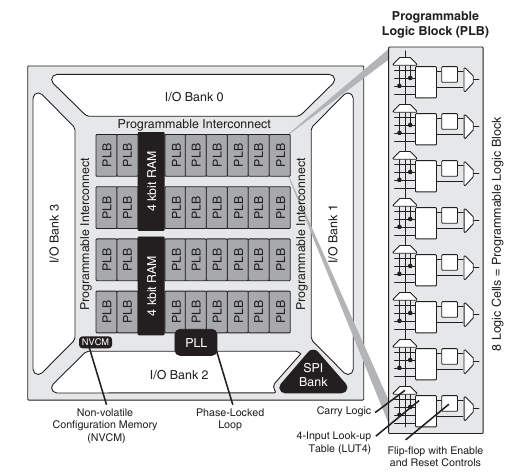
\includegraphics[width=0.80\textwidth]{../figures/iCE40_block_diagram.png}
	\caption[Blockdiagramm des verwendeten iCE40 FPGAs]{Aufbau des verwendeten iCE40 FPGAs (Quelle: iCE40 Datasheet{\cite{doc:datasheet}})}
	\label{fig:ice40_block_diagram}
\end{figure}

Zusätzlich ist die Anzahl von Funktionsblöcken bei FPGAs üblicherweise deutlich höher als als bei CPLDs, weswegen in dieser Arbeit ein FPGA-Chip verwendet werden soll.

Die in der Abbildung erkennbaren I/O-Bänke beinhalten GPIO-Pins die als Ein- oder Ausgänge konfiguriert und direkt mit den Logikblöcken (``PLBs'') im FPGA verbunden werden können.

\subsection{Datenzwischenspeicher: SRAM}

Nach der Erfassung müssen die Daten zwischengespeichert werden. Dabei sind vor allem zwei Faktoren entscheidend:
\begin{itemize} 
	\item Die \textbf{Geschwindigkeit} des Speichers, die meist den maximalen Datendurchsatz der Gesamtschaltung bestimmt
	\item Die \textbf{Größe} des Speichers, die festlegt wie lange bei hohem Datendurchsatz aufgenommen werden kann 
\end{itemize}
Die meisten nicht-flüchtigen Speicher sind aufgrund der unzureichenden Geschwindigkeit nicht für diesen Verwendungszweck geeignet, weswegen sich die Verwendung von \acrshort{RAM}-Speicher anbietet. \\
Bei Mikrocontrollern und kleineren FPGA-Boards werden aus Kostengründen und wegen der unkomplizierten Ansteuerung oft SRAM-Speichereinheiten verbaut. SRAM-Speicher hat meist sehr kurze Zugriffszeiten, allerdings bei einer geringen Speichergröße von wenigen MBit. Der in dieser Arbeit verwendete SRAM-Speicher hat beispielsweise eine Größe von 4 Mbit (512 KB) und könnte damit 62500 Events zwischenspeichern\footnote{Bei einer angenommenen Event-Größe von 64-Bit, und unter der Annahme dass der SRAM-Speicher ausschließlich zum Zwischenspeichern von Events verwendet wird}.\\
Bei kontinuierlicher Erfassung von Eingangssignalen mit einer Abtastrate von 100 Mhz entspricht dies einer Aufnahmezeit von unter einer Millisekunde\footnote{$62500 * 10 ns = 0.625 ms$}. Da allerdings keine Eingangssignale erwartet werden, bei denen Events mit einer Frequenz von 100 Mhz auftreten und außerdem bereits bei laufender Aufnahme Events aus dem RAM-Speicher entnommen und weiter übertragen werden, kann der SRAM-Speicher trotzdem im Sinne der Aufgabenstellung als Zwischenspeicher verwendet werden.\\
Als Alternative könnte DRAM-Speicher verwendet werden, der ein Vielfaches der Speicherkapazität bietet und damit auch längere Aufnahmen bei hoher Signaldichte ermöglichen würde. DRAM-Speicher erfordert allerdings im Vergleich zu SRAM ein kontinuierliches ``Auffrischen'' der Speicher-Inhalte durch eine Controller-Einheit und bedeutet dementsprechend deutlich mehr Aufwand und hohe Timinganforderungen bei der Implementierung.


\subsection{Datenübertragung: SPI}

Nach der Datenerfassung und Zwischenspeicherung werden die Daten an ein externes System übertragen, an dem sie weiterverarbeitet oder ausgewertet werden können. Zur Datenübertragung gibt es eine Vielzahl von Schnittstellen und Protokollen. Dabei werden die Daten im Normalfall ``serialisiert'', das heißt wenn ein Event aus 64 Bits besteht, werden die Bits nacheinander über eine einzige Datenleitung übertragen. Geläufige serielle Datenübertragungsverfahren sind vor allem \acrshort{UART}, \acrshort{I2C} und \acrshort{SPI}.
\begin{description}
	\item Bei einem \textbf{UART (\acrlong{UART})} werden die Daten über eine Empfangs- und eine Sendeleitung ausgetauscht. Es wird kein eigenes Taktsignal übertragen, weswegen auf beiden Seiten eine feste Übertragungsgeschwindigkeit (``Baud-Rate'') eingestellt werden muss. UART-Schnittstellen sind weit verbreitet und verhältnismäßig einfach zu implementieren, dabei allerdings recht fehleranfällig und bei üblichen Baud-Raten ist die Übertragungsgeschwindigkeit stark limitiert (vgl. \cite{wiki:UART}).
	\item \textbf{\acrshort{I2C} (\acrlong{I2C})} ist ein synchroner Datenbus, bei dem eine eigene Leitung für den Takt und eine Datenleitung verwendet wird. $\text{I}^2$C arbeitet nach dem Master-Slave-Prinzip, das heißt es können auch mehrere Geräte miteinander kommunizieren. $\text{I}^2$C untertützt Übertragungsraten bis zu 5 Mbit/s (unidirektional, vgl. \cite{wiki:I2C}).
	\item \textbf{\acrshort{SPI} (\acrlong{SPI})} ist wie $\text{I}^2$C ein synchroner Datenbus nach dem Master-Slave-Prinzip. Neben der Leitung für den Takt wird eine Daten-Leitung in Senderichtung und eine Datenleitung in Empfangsrichtung verwendet. Zusätzlich wird pro Gerät eine ``Chip-Select'' Leitung benötigt, um die Geräte adressieren zu können. SPI kann Übertragungsraten bis in den mehrstelligen Megabit-Bereich ermöglichen (vgl. \cite{wiki:SPI}).
\end{description}

Aufgrund der hohen Übertragungsrate und der relativ unkomplizierten Implementierungsmöglichkeiten soll SPI für die Datenübertragung verwendet werden.


\subsection{Steuerung der Aufnahme und sequentielle Programmabläufe}

Neben der reinen Datenerfassung und -Übertragung werden noch Komponenten zur Steuerung und zur Kontrolle des Aufnahmevorgangs benötigt.\\
Grundsätzlich können die benötigten Vorgänge- und Zustände (zum Beispiel das Starten und Stoppen der Aufnahme) direkt im FPGA umgesetzt werden. Als Kommunikationsweg zur Steuerung und Konfiguration kann dann wiederum SPI verwendet werden.\\
Bei längeren oder komplexeren Programmabläufen die keine zeitkritische Ausführung erfordern bietet sich die Verwendung eines zusätzlichen Mikrocontrollers an. Da die meisten PC-Systeme keine programmierbaren \acrshort{GPIO}-Pins als SPI-Schnittstelle zur Verfügung stellen, kann ein Mikrocontroller außerdem als Brücke zwischen FPGA und Anwendersystem fungieren, und zum Beispiel die vom FPGA erfassten Daten über einen USB-Port zur Verfügung stellen.\\
Davon abgesehen wird unter Umständen noch zusätzliche Hardware- und Software-Infrastruktur benötigt um das FPGA und den Mikrocontroller zu programmieren und zu konfigurieren.
\clearpage

\section{Auswahl der Software-Toolchain: IceStorm}

Im Normalfall werden FPGAs mit den vom Hersteller angebotenen Software-Tools programmiert. Bei diesen Tools handelt es sich um kommerzielle Produkte bei denen zum Teil auch hohe Lizenzgebühren fällig werden. Da der Quelltext dieser Tools nicht öffentlich zugänglich ist und FPGA-Hersteller keine relevanten Informationen zur Hardwarestruktur von FPGA-Chips veröffentlichen war es für Opensource-Tools bisher nicht möglich eine Alternative zu den kommerziellen Toolchains der Hersteller zu bieten.\\
Mit der IceStorm-Toolchain wurde erstmals die Hardwarestruktur der -- relativ einfach aufgebauten -- Lattice iCE40 Produkt-Serie\footnote{Es werden nicht alle Chips der iCE40-Serie unterstützt, die verwendbaren Produktvarianten sind auf der IceStorm-Website aufgelistet\cite{web:IceStorm}} durch \gls{Reverse-Engineering} rekonstruiert, so dass ein vollständiger Arbeitsablauf für die Entwicklung von FPGA-Designs zur Verfügung steht.\\
Der Arbeitsablauf lässt sich in mehrere grundlegende Schritte unterteilen:
\begin{itemize}
	\item Erstellen des Quelltexts für ein FPGA-Design in einer Hardwarebeschreibungssprache wie \gls{Verilog} oder \acrshort{VHDL}
	\item Prüfung der Funktion des Designs mit einem Software-Simulator
	\item Synthese des Designs: Der Quelltext wird in Funktionsblöcke umgewandelt die durch Hardware-Komponenten des FPGAs (wie Ein- und Ausgänge, Lookup-Tabellen für logische Funktionen, FlipFlops oder BRAM als Speichereinheiten, etc.) realisiert werden können
	\item ``Place-and-Route'': Es wird eine geometrische Anordnung der Funktionsblöcke auf dem FPGA-Chip entworfen (``place'') und die Einzelkomponenten werden miteinander verbunden (``route''). Dabei müssen auch die zeitlichen Anforderungen der Schaltung berücksichtigt werden.
	\item Abschließend wird das Ergebnis des ``Place-and-Route''-Vorgangs in ein Format gebracht mit dem direkt die Hardware konfiguriert werden kann -- dem sogenannten ``Bitstream'' -- und das Bitstream wird auf den FPGA-Chip übertragen
\end{itemize}

Die IceStrom-Toolchain bildet diesen Ablauf folgendermaßen ab:

\begin{itemize}
	\item Als Hardwarebeschreibungssprache wird Verilog unterstützt\footnote{Zum Zeitpunkt der Erstellung dieser Arbeit gibt es kein vollständiges VHDL-Frontend für das Synthese-Tool {\tt yosys}. Mit dem Projekt ``YODL'' wurde eine Implementierung begonnen, die aber seit längerem nicht mehr weiterentwickelt wird (siehe \cite{web:yodl}). Davon abgesehen können VHDL-zu-Verilog Konverter verwendet werden, wobei allerdings nicht immer von einer problemfreien Konvertierung ausgegangen werden kann} 
	\item Die IceStorm-Toolchain enthält kein eigenes Tool für die Simulation, es können aber existierende Lösungen wie zum Beispiel {\tt iverilog}\cite{web:iverilog} und {\tt gtkwave}\cite{web:gtkwave} (zur grafischen Darstellung der Simulationsergebnisse) verwendet werden
	\item Als Synthese-Tool dient {\tt yosys}\cite{web:yosys}
	\item Für den Pace-and-Route-Vorgang wird {\tt arachne-pnr}\cite{web:arachne_pnr} verwendet
	\item Für die Generierung und das Übertragen des Bitstreams stehen als Teil der IceStorm-Tools\cite{web:icestorm_tools} {\tt icepack} und {\tt iceprog} zur Verfügung
\end{itemize}



\subsection{IcoSoc als Prototyping- und Implementierungsplattform} 

Vom selben Autoren\footnote{Die Entwicklung der IceStorm-Toolchain wurde vor allem von Clifford Wolf vorangetrieben, das Projekt hat aber auch eine aktive Community die regelmäßig Beiträge leistet} wie das Synthese-Tools {\tt yosys} gibt es mit dem {\tt picorv32} auch eine RISC-V CPU-Implementierung in Verilog und mit dem {\tt IcoSoc}-Projekt eine Softwareumgebung die auf die einfache Verwendung des {\tt picorv32}-Prozessors auf einem iCE40-basierten Entwicklungs-Board (``IcoBoard'') ausgerichtet ist. Das {\tt IcoSoc}-Projekt liefert eine Reihe von Modulen, mit denen zum Beispiel die Daten der GPIO-Pins direkt in den SRAM-Speicher gemappt werden können, oder die die Kommunikation mit externer Hardware (zum Beispiel über SPI oder UART) ermöglichen. Es werden also typische Mikrocontroller-Funktionalitäten direkt auf dem FPGA umgesetzt und es kann mit RISC-V kompatiblem C-Quellcode gearbeitet werden, wodurch viele Implementierungs-Aufgaben deutlich erleichtert werden. Dabei allerdings mit dem Nachteil dass die ``Soft-CPU'' auf dem FPGA-Board nur mit der vergleichsweise langsamen Geschwindigkeit von circa 20 Mhz läuft, und dementsprechend keine unmittelbar zeitkritischen Vorgänge übernehmen kann.\\
Das {\tt IcoSoc}-Projekt wurde für diese Arbeit auf das verwendete FPGA-Board portiert, um Funktionsabläufe zu testen und weniger zeitkritische Abläufe zu implementieren.



\section{Auswahl der Hardware}

\subsection{IceZero FPGA-Shield (iCE40HX4K)}

Die Auswahl der Toolchain schränkt die verwendbare FPGA-Hardware auf die unterstützten iCE40-Modelle ein.
Aufgrund des kompakten Formfaktors und des vergleichsweise günstigen Preises wurde das IceZero-FPGA-Shield für die Aufgabenstellung ausgewählt.
Der auf dem IceZero-Board verwendete ``ÌCE40HX4K''-Chip (im TQ144-Formfaktor) bietet 107 programmierbare Ein- bzw. Ausgangspins und laut Datenblatt 3520 ``Logic Cells''. 
Hardware-seitig hat der Chip allerdings den gleichen Funktionsumfang wie das größere ``8K''-Model -- die Limitierung auf 3520 Logic Cells  wird durch eine Software-Sperre der vom Hersteller zur Verfügung gestellten ``iCEcube2''-Toolchain erreicht.\\
Das heißt bei Verwendung mit der IceStorm-Toolchain bietet der Chip den gleichen Funktionsumfang wie die im Datenblatt abgebildete 8K-Variante:

\begin{table}[H]
\centering
\begin{tabular}{|l|l|c|c|}
\hline
\rowcolor[HTML]{EFEFEF} 
\textbf{Part Number}             & {[}...{]} & \multicolumn{1}{l|}{\cellcolor[HTML]{EFEFEF}\textbf{HX4K}} & \multicolumn{1}{l|}{\cellcolor[HTML]{EFEFEF}\textbf{HX8K}} \\ \hline
Logic Cells (LUT + Flip-Flop)    &           & 3,520                                                      & 7,680                                                      \\ \hline
RAM4K Memory Blocks              &           & 20                                                         & 32                                                         \\ \hline
RAM4K RAM bits                   &           & 80K                                                        & 128K                                                       \\ \hline
Phase-Locked Loops (PLLs)        &           & 2                                                          & 2                                                          \\ \hline
Maximum Programmable I/O Pins    &           & 95                                                         & 206                                                        \\ \hline
Maximum Differential Input Pairs &           & 12                                                         & 26                                                         \\ \hline
High Current LED Drivers         &           & 0                                                          & 0                                                          \\ \hline
\end{tabular}
	\caption{Hardware-Spezifikationen des verwendeten iCE40HX4K-Chips (vgl. \cite{doc:datasheet})}
\label{tbl:ice40_specs}
\end{table}

Vom FPGA-Chip selbst abgesehen beinhaltet das IceZero-Board einen 4MBit (512KB) großen SRAM-Speicher und einen 64MBit (8MB) großen SPI-Baustein, der zur Speicherung des Bitstreams und der Konfiguration des FPGAs verwendet werden kann.
Es ist ein 100Mhz schneller Oszillator zur Erzeugung des Systemtakts verbaut und es sind drei benutzerprogrammierbare LEDs vorhanden.
Die vorhandenen Ein- und Ausgänge liegen an 4 \gls{PMOD}-Schnittstellen und einer 40-Pin-Buchsenleisten für den Anschluss an ein Raspberry Pi an (siehe \cite{web:trenz_icezero}). 


\subsection{Raspberry Pi Zero W}

Das IceZero-Board ist für die Verwendung mit einem Raspberry Pi-Mikrocontroller vorgesehen und hat den gleichen Formfaktor wie das Raspberry Pi Zero (mit circa 5 x 3 cm das kleinste Modell der Raspberry Pi Serie).\\
Das Raspberry Pi dient für diese Arbeit hauptsächlich dem Zweck über die mit dem FPGA verbundenen GPIO-Pins eine Schnittstelle für die Konfiguration und den Datenaustausch mit dem FPGA zu liefern.\\
Prinzipiell steht mit dem Raspberry Pi ein Mikrocontroller mit großem Funktionsumfang und Leistungsreserven zur Verfügung, mit dem weitergehende Funktionen umgesetzt werden könnten. 
Das Raspberry Pi kann per USB direkt an einen Anwender-PC angeschlossen werden und könnte mithilfe verschiedener USB-Modi zum Beispiel als Netzerkgerät eine Web-Seite mit einer grafischen Darstellung der Ergebnisse anzeigen, oder als serielle Schnittstelle das SUMP2-Protokol zur Weitergabe der Aufnahme-Daten an den Anwender-PC implementieren. 

\clearpage

\section{Beispiel: Von der Synthese bis zum Bitstream mit der IceStorm-Toolchain}
\clearpage


     
\chapter{Implementierung}
\label{ch:Implementierung}

Grundlage für die Arbeit mit dem FPGA-Board ist eine Möglichkeit generierte Bitstreams auf das FPGA-Board zu übertragen.
Auf der Produkt-Seite des Herstellers des IceZero-Boards (Trenz Electronic)\cite{web:trenz_icezero}wird für diesen Zweck auf das Git-Repository des {\tt icotools}-Projekts verwiesen, in dem sich ein einfaches Testbeispiel zur Überprüfung des SRAM-Speichers befindet -- und das C-Programm {\tt icezprog} zum Flashen des Bitstreams.\\
Das {\tt icezprog}-Programm implementiert über direktes Ansprechen von GPIO-Pins (``bit-banging'') eine SPI-Schnittstelle zum Flash-Speicher des IceZero-Boards, und nach einem Neustart{\footnote{Der Neustart wird durch setzten des mit dem FPGA verbundenen GPIO-Pins ``CONFIG\_RESET'' ausgeführt} konfiguriert sich das FPGA selbständig mit dem Inhalt des auf dem Flash-Speicher abgelegten Bitstreams.\\
Für die spätere Verwendung des {\tt IcoSoc}-Projekts wird allerdings noch weitere Funktionalität benötigt. Wichtig ist hier vor allem die Möglichkeit Speicherinhalte mit einem ``Offset'' in den Flash-Speicher zu schreiben, da später zusätzlich zum Bitstream auch ein ``appimage'' auf dem Flash-Speicher abgelegt wird, das den auszuführenden C-Code für den {\tt IcoSoc} enthält.\\
Das {\tt icotools}-Projekt enthält mit dem Tool {\tt icoprog} ein Programm das (unter anderem) Offsets unterstützt und in erster Linie zum Programmieren von Bitstreams für das IcoBoard gedacht ist. IcoSoc unterstützt außerdem Debugging-Funktionalitäten die über eine eigene 10 Bit breite parallele Schnittstelle zum Raspberry Pi realisiert sind. Diese Schnittstelle kann auch verwendet werden um ein {\tt appimage} beim Start des IcoSocs direkt zu laden, ohne dass es vorher im Flash-Speicher abgelegt werden muss. Die Schnittstelle wird ebenfalls über das {\tt icoprog}-Tool angesprochen.\\
Um die selbe Funktionalität auch für das IceZero-Board zur Verfügung zu stellen wurde als erstes das {\tt icoprog}-Tool entsprechend angepasst. 

\section{Anpassung des Tools zum Programmieren des Bitstreams (icoprog)}
\label{ch:Implementierung:sec:icoprog}

Das IcoBoard verfügt wie das IceZero-Board über einen 40-Pin-Header zum Anschluss an ein Raspberry Pi. Davon abgesehen kann das IcoBoard aber auch mit einem zusätzlichen FTDI-Interfaceboard über USB programmiert werden. Das {\tt icoprog}-Programm enthält deswegen sowohl Methoden zur Programmierung via USB als auch über die GPIO-Pins des Raspberry Pis, und noch eine zusätzliche GPIO-basierte Variante für ein anderes Board. Ursprünglich war geplant eine Konfiguration für das IceZero-Board direkt in das icoprog-Tool zu integrieren, aufgrund der ohnehin schon unübersichtlichen Code-Basis wurden die benötigten Komponenten aber in ein eigenes Programm namens {\tt icozctl} ausgelagert, dass dann später um Funktionen zur Steuerung der Aufnahme und Datenübertragung erweitert wurde.\\ 
Für die Anpassung mussten einige GPIO-Pins geändert werden, da beim IceZero-Board nicht alle Pins der GPIO-Headers mit dem FPGA verbunden sind. (Das IcoBoard verwendet einen iCE40-Chip im CT256-Formfaktor, weswegen deutlich mehr Pins zur Verfügung stehen als beim IceZero-Board\cite{web:trenz_icoboard}).\\
Davon abgesehen ist auf dem IcoBoard ein zusätzlicher MachXO2-Chip von Lattice verbaut, der (unter anderem) das SPI-Signal vom Raspberry Pi je nach gesetztem Chip-Select-Signal entweder direkt an das FPGA oder den Flash-Speicher weiterleitet. Beim IceZero-Board sind das FPGA und der Flashspeicher direkt an die gleichen GPIO-Pins des Raspberry Pis angeschlossen (inklusive Chip-Select-Signal), ein gezieltes Ansprechen der einzelnen Komponenten ist deswegen nicht möglich, und die entsprechenden Chip-Select-Signale wurden aus dem Code entfernt. 
Im späteren Verlauf der Implementierung wurde entschieden die parallele Schnittstelle zu entfernen, da mit ihr keine bidirektional Kommunikation mit der nötigen Geschwindigkeit realisiert werden konnte. Stattdessen wurde mit den frei-gewordenen Pins eine SPI-Schnittstelle und ein zusätzlicher UART für einfache Debug-Ausgaben umgesetzt.\\
Ein direktes Flashen von {\tt appimages} beim Starten des IcoSoc ist dementsprechend bei aktuellem Stand nicht möglich und die erweiterten Debug-Funktionen des IcoSoc sind nicht verfügbar. 
Davon abgesehen kann das {\tt icozctl}-Tool auf dem IceZero-Board mit der gleichen Syntax wie {\tt icoprog} für das IcoBoard verwendet werden.
Zu Debug-Zwecken wurde {\tt icoprog} außerdem um eine Option ``-N'' erweitert, mit der ein Offset für das Auslesen des aktuellen Flash-Speicher-Inhalts angegeben werden kann.

\section{Portierung und nötige Anpassungen des Verilog-SoCs (IcoSoc)}
\label{ch:Implementierung:sec:icosoc}
Als nächstes wurde das IcoSoc-Projekt auf das IceZero-Board portiert. 

\subsection{Struktur des IcoSoc-Projekts}
Zum Überblick soll erst ein kurzer Blick auf die Verzeichnisstruktur des Projekts geworfen werden:
\begin{minted}{bash}
./common
./common/firmware.c
./common/firmware.S
./common/icosoc_debugger.v
./common/icosoc_raspif.v
./common/picorv32.v
./common/riscv_flash.ld
[...]
./examples
./examples/event_recorder
./examples/hello
[...]
./mod_gpio
./mod_rs232
./mod_spi
[...]
./README
./icosoc.py
\end{minted}

Im Verzeichnis {\tt common/} befinden sich die Grundbausteine des IcoSoc-Systems. Dazu gehört die Verilog-Implementierung des PicoRV32-Prozessors und weitere grundlegende Systemkomponenten wie zum Beispiel die erwähnte Raspberry Pi Schnittstelle (``raspif'') und außerdem die nötige Firmware zum Starten des IcoSocs und zum Laden der {\tt appimages}. Zusätzlich findet sich hier auch das benötigte Linker-Skript für den C-Code der {\tt appimages}.\\
Im Verzeichnis {\tt examples/} liegen verschiedene Beispiel-Projekte, unter anderem ein ausführliches ``Hello world''-Beispiel in dem die für IcoSoc-Projekte verfügbaren Komponenten vorgestellt werden -- und das in dieser Arbeit entworfene Event-Recorder Projekt.\\
Darauf folgen die verfügbaren IcoSoc-Module jeweils in einem eigenen Unterverzeichnis.\\
Das Modul ``mod\_gpio'' stellt zum Beispiel die Funktionalität zur Verfügung, das im C-Code GPIO-Pins als Ausgänge definiert werden können und ihr Ausgangspegel anschließend über das Schreiben an eine bestimmte Speicheradresse gesetzt werden kann. 
Zuerst muss das Modul in der Projekt-Konfigurationsdatei {\tt icosoc.cfg} aktiviert werden:
\begin{minted}{python}
board icoboard
mod gpio gpios
    address 2
    connect IO pmod2 pmod1
\end{minted}

Die Benutzung im C-Code würde dann folgendermaßen aussehen:

\begin{minted}{c}
// Alle GPIO Pins als Ausgang verwenden
icosoc_gpios_dir(0xffff);

// Ersten Pin auf '1' setzen
icosoc_gpios_set(0x0001);
\end{minted}

Wobei der ``set''-Befehl des Moduls als einfacher Schreibbefehl an eine Speicheradresse implementiert ist:
\begin{minted}{c}
static inline void icosoc_@name@_set(uint32_t bitmask) {
    *(volatile uint32_t*)(0x20000000 + @addr@ * 0x10000) = bitmask;
}
\end{minted}

Die Module selbst sind in Verilog geschrieben und bilden somit eine Brücke zwischen dem Timing-stabilen Verilog-Teil und dem langsameren C-Code.\\

Direkt im Projekt-Verzeichnis findet sich eine README-Datei und das Python-Skript {\tt icosoc.py}.
Das Python-Skript generiert aus der Projekt-Konfigurationsdatei mithilfe der verfügbaren Module und Grundkomponenten den eigentlichen Verilog-Code für den IcoSoc und kümmert sich um die ordnungsgemäße Verbindung und Konfiguration der Module. (Die Platzhalter ``@name@'' und ``@addr@'' in der Definition der {\tt gpio\_get()}-Methode werden hier zum Beispiel auch durch die in der Konfigurationsdatei festgelegten Werte ersetzt).
Zusätzlich wird ein {\tt Makefile} generiert, mit dem das Projekt synthetisiert, der C-Code kompiliert, und abschließend der erzeugte Bitstream und das {\tt appimage} auf das FPGA-Board geflasht werden können.

\subsection{Portierung des IcoSoc-Projekts}

Für die Portierung waren gemäß der Struktur des IcoSoc-Projekts hauptsächlich Anpassungen im {\tt icosoc.py} Skript nötig.\\
Das Python-Skript generiert unter anderem auch die {\tt icosoc.pcf}-Datei, in der die Pin-Definitionen für die Synthese festgelegt werden.
Da auf dem IceZero-Board ein anderes iCE40-FPGA-Modell verwendet wird, mussten hier alle Pin-Definitionen gemäß den Informationen aus dem IceZero-Board-Schaltplan\cite{doc:schematic} angepasst werden.
Ein einfaches Beispiel wäre der Eingang des Systemtakts und die LED-Pins: 
\begin{minted}{python}
if board == "icezero":
    icosoc_pcf["10-std"].append("""
    set_io CLKIN  49  // icoboard: R9
    set_io LED1   110 // icoboard: C8
    set_io LED2   93  // icoboard: F7
    set_io LED3   94  // icoboard: K9
[...]
""")
\end{minted}

Wie im Beispiel ersichtlich ist wurden die meisten durchgeführten Änderungen mit der Variable ``board''  parameterisiert, so dass die Unterstützung mehrerer Board mit vergleichsweise geringem Aufwand möglich wäre\footnote{Für die Untersützung mehrerer Boards wäre eine tiefergehende Umstrukturierung des IcoSoc-Projekts sinnvoll, die aber über den Umfang dieser Arbeit hinausgeht}.

Die PMOD-Pins werden den verwendeten Modulen nach Bedarf zugewiesen und nach einem festen Namensschema benannt (siehe hierzu auch ``\nameref{sec:pmod_all}'').\\
Auch hier wurden die entsprechenden Pin-Definitionen angepasst.\\
Für IcoSoc-Module sind grundsätzlich nur Verbindungen zu PMOD-Pins vorgesehen. Für die geplante Funktionalität werden allerdings auch Verbindungen zu anderen FPGA-Pins und Verilog-Signalen (wie zum Beispiel dem CLKIN Pin) benötigt. Das Skript wurde so angepasst, dass Moduldefinitionen auch andere -- in einer Liste festgelegte --  Signale verwenden dürfen.
\begin{minted}{python}
def make_pins(pname):
    [...]
    allowed_signals = ['CLKIN']
    if pname in allowed_signals:
        return [pname]
    [...]
\end{minted} 

Wie schon erwähnt wurde außerdem die ``RASPIF''-Schnittstelle entfernt, und stattdessen ein einfacher UART für Debug-Ausgaben integriert.\\
Die Änderungen wurden analog zu einem {\tt icotools}-Fork\footnote{Der Fork enthält außerdem zusätzliche Beispiel-Projekte und unter anderem ein I$^2$C-Modul} auf Github durchgeführt, bei dem die gleichen Anpassungen für ein anderes iCE40-basiertes Board durchgeführt wurden (``BlackIce II''-Board, siehe \cite{web:lawrie_fork}). \\
Davon abgesehen wurde ein unbenutztes ``HRAM''-Signal aus dem Design entfernt und kleinere Änderungen an der Generierung des Makefiles durchgeführt. Der {\tt icoprog}-Befehl wurde durch {\tt icozctl} ersetzt und das Log-Level wurde auf die Stufe ``-v2'' reduziert. Außerdem muss dem Place-and-Route-Befehl ({\tt arachne-pnr}) und der durchgeführten Timing-Analyse ({\tt icetime}) mit der Option {\tt -P tq144:4k} der Formfaktor des iCE40-Chips mitgegeben werden, damit die Pindefinitionen richtig zugeordnet werden können.   
Mit den genannten Änderungen liegt ein voll funktionsfähiger Port des IcoSoc-Projekts für das IceZero-Board vor.

\section{Implementierung des Event-Recorder Moduls}
\label{ch:Implementierung:sec:Event-Recorder}

Zur Implementierung der Signalerfassung wurde ein eigenes IcoSoc-Modul namens {\tt mod\_triggerrec} erstellt.
\subsection{GPIO-Eingänge}
Die Erfassung der an den PMOD-Headern anliegenden Eingangssignale erfolgt analog zum GPIO-Modul, allerdings mit dem Unterschied dass die verwendeten Pins fest als Eingänge definiert werden.
Dafür wird bei der Instantiierung des SB\_IO-Primitves für den PIN\_TYPE die Bit-Kombination {\tt 0000\_01} gesetzt (siehe ``Input Pin Function Table'' aus der SiliconBlue ICE Technology Library\cite[S.~73]{doc:tec_lib}).\\ 
Auf den Registerinhalt des so definierten SB\_IO-Primitives kann dann in Verilog mit einem einfachen ``wire'' der entsprechenden Bit-Breite zugegriffen werden:
\begin{minted}{verilog}
// gpio input
wire [IO_LENGTH-1:0] io_in;
\end{minted}

\subsection{Bus-Schnittstelle}
Um Daten aus dem Verilog-Teil in den C-Teil transferieren zu können muss die Bus-Schnittstelle des IcoSoc in Verilog implementiert werden.
Dafür werden -- wie im GPIO-Modul -- die Signale {\tt ctrl\_rd}, {\tt ctrl\_wr}, {\tt ctr\_addr} und {\tt ctrl\_wdat} als Eingänge {\tt ctrl\_rdat} und {\tt ctrl\_done} als Ausgänge des Moduls zur Verfügung gestellt.
Die Bus-Schnittstelle wird (vereinfacht) folgendermaßen umgesetzt:
\begin{minted}{verilog}
always @(posedge clk) begin		
	if (!ctrl_done) begin
		ctrl_done <= 1;
		// write from bus to local register associated with address 4
		if (|ctrl_wr) begin
			if (ctrl_addr == 4) local_register <= ctrl_wdat;
		end
		// read from local registers to bus
		if (ctrl_rd) begin
			if (ctrl_addr == 4) ctrl_rdat <= local_register;
		end
	end
end
\end{minted}

Für die meisten Register wird eine Länge von 64 Bit verwendet. Da der Bus eine Breite von 32 Bit hat (also nur 32 Bit in einem Takt übertragen kann), wird für diese Register eine zusätzliche Zustandsvariable ({\tt ctrl\_state}) verwendet, so dass beim ersten Zugriff immer die höheren 32 Bit übertragen werden und beim zweiten Zugriff (und zweiten Zustand) die unteren 32 Bit.. 

\subsection{BRAM-Speicher für die Event-Definitionen}

Da aus dem Verilog-Modul ein direkter Zugriff auf die Event-Definitionen und -Trigger möglich sein soll werden diese in einem Register-Array abgelegt.\\
Die Länge des Arrays ist parametrisiert, so dass die Anzahl der gewünschten Event-Trigger bei der Synthese angegeben werden kann. Bei einfacher Lese- und Zugriffs-Logik wird das Array als BRAM synthetisiert wird, und es werdem damit keine zusätzlichen `Logic Slices' in Anspruch genommen.\\  
Im Trigger-Array werden die 64 Bit langen Event-Definitionen jeweils in zwei aufeinander-folgende 32-Bit Werte aufgeteilt, da dies die Bus-Logik etwas vereinfacht.  
Bei der Bus-Kommunikation wird die angeforderte Adresse ({\tt ctrl\_addr}) mit einem Offset\footnote{Die Adresse hat um der Bitbreite der Registerelemente zu entsprechen einen ``Multiplikator'' und wird deswegen zusätzlich per Rechts-Shift verkleinert bevor der Index generiert werden kann} in den Index des Event-Registers-Arrays umgesetzt, so dass alle Array-Elemente direkt vom Bus ansprechbar sind. 

\subsection{Erkennung von Signaländerungen und Events}

Der erste Schritt bei der Auswertung des GPIO-Registers ist die kontinuierliche Erkennung von Signaländerungen.\\
Dies wird im Verilog-Code durch einen einfachen Vergleich und ein Zwischenspeichern des alten Signalzustands erreicht:

\begin{minted}{verilog}
	// input capture
	always @(posedge clk_fast) begin
		// increment counter if active
		if (status[0])  
			counter <= counter + 1;
		
		// on input changes ..
		if ((io_buf2 != io_buf1)) begin
			data_in_fast <= { io_buf1, 1'b0, counter[46:0] };
			shift_in_fast <= 1;
		end
	end
	
	io_buf1 <= io_in;
	io_buf2 <= io_buf1;	
	[...]

\end{minted}
An dieser Stelle wird auch der Zähler erhöht, wenn das Modul in aktiviertem Zustand ist.\\
Darüber hinaus wurde auch eine Event-Erkennung in Verilog begonnen. Bei der vorhandenen Implementierung wird bei der Synthese allerdings eine große Menge kombinatorischer Logik generiert, und es können nicht ausreichend viele Event-Definitionen umgesetzt werden (Die Kapazität des iCE40-Chips wird bei circa 8 Event-Definitionen erreicht, bei großer Auslastung der Logic Slices erhöhen sich auch die Place-and-Route-Zeiten auf Werte von einer halben Stunde oder mehr). \\
Ohne weitere Optimierungen ist die Event-Erkennung in Verilog deswegen nicht praktikabel und wurde bei aktuellem Stand der Arbeit wieder deaktiviert.\\
Es ist anzumerken, dass die Erkennung von Signaländerungen das Datenvolumens bei der Aufnahme bereits stark reduziert -- insbesondere bei geringer Signaldichte.

\subsection{Cross-Clock BRAM-Puffer}

Da die Event-Erkennung im Verilog-Teil noch nicht abgeschlossen ist, aber auch um schnell aufeinander-folgende Signale ohne Verlust erfassen zu können, macht es Sinn bereits direkt auf dem FPGA ein Puffer für die Aufnahmedaten zu implementieren. Der Puffer soll wiederum als BRAM synthetisiert werden, da es sich um größere Datenmengen handelt und keine kombinatorische Logik verbraucht werden soll.\\
Bei FPGA-Implementierungen werden derartige Puffer häufig benötigt -- und dabei oft mit der zusätzlichen Funktionalität, dass Daten zwischen unterschiedlich schnell getakteten Komponenten ausgetauscht werden. Der Austausch von Daten zwischen verschiedenen Taktdomänen ist dabei kein triviales Problem. Das {\tt IcoSoc}-Projekt enthält in der Datei {\tt icosoc\_crossclockfifo.v} allerdings bereits eine Implementierung eines solchen Cross-Clock-Puffers, die für das {\tt raspif}-Modul verwendet wird. Da keine weitere Dokumentation zum Puffer-Modul vorhanden ist, wurde zuerst eine {\tt iverilog}-Testbench geschrieben, die die erwartete Funktionsweise bestätigt hat. Das {\tt crossclockfifo}-Modul konnte so erfolgreich als BRAM-Puffer in das Event-Recorder-Modul eingebunden werden.\\
IcoSoc-Module laufen im Normalfall mit dem Systemtakt des IcoSocs. Dieser wird durch eine PLL-Konfiguration generiert und liegt bei (circa) 20 Mhz.\\
Zusammen mit der bei der Portierung des {\tt IcoSoc}-Projekts durchgeführten Anpassung, dass IcoSoc-Module auch andere Ein- und Ausgänge als die PMOD-Pins haben können, konnte so das 100 Mhz schnelle CLKIN-Signal an das Event-Recorder-Modul weitergereicht werden und damit eine Steigerung der Erfassungsgeschwindkeit auf 100 Mhz erreicht werden.  

\subsection{Simulation des Event-Recorder-Moduls mit iverilog}

Das Verhalten des Event-Recorder-Moduls lässt sich mit einer {\tt iverilog}-Testbench simulieren.\\
Durch die Bus-Schnittstelle kann dabei die erwartete Funktionalität geprüft werden ohne die anderen Komponenten des {\tt IcoSoc}-Systems mitsimuliert werden  müssen.

In der Testbench werden zwei ``tasks'' für den schreibenden und lesenden Bus-Zugriff erstellt, deren Verhalten einem tatsächlichen Bus-Zugriffs entspricht:

\begin{minted}{verilog}
	task ctrl_write(input [15:0] addr, input [31:0] data); begin
		ctrl_wr <= 1;
		ctrl_rd <= 0;
		ctrl_addr <= addr;
		ctrl_wdat <= data;
		@(posedge clk);
		while (!ctrl_done) @(posedge clk);
		ctrl_wr <= 0;
	end endtask

	task ctrl_read(input [15:0] addr); begin
		[...]
	end endtask
\end{minted}

Anschließend können in der Testbench Speicher-Zugriffe -- analog zu den vom Modul definierten C-Funktionen -- simuliert werden und ihr Ergebnis geprüft werden.
\begin{minted}{verilog}
		// test write to status register (address 0x04)
		ctrl_write('h4, 'h01); 
		repeat (2) @(posedge clk);
		
		// read status register
		ctrl_read('h4);	
		repeat (2) @(posedge clk);
		
		$display("Status: %s", (ctrl_rdat == 'h01)? "OK" : "Not OK");                                                    //$	

\end{minted}

Für die Ausführung der Testbenches ist jeweils ein kurzes Bash-Skript vorhanden, so kann im Modul-Verzeichnis {\tt mod\_triggerrec} zum Beispiel der Befehl
\begin{minted}{bash}
sh testbench.sh
\end{minted}
ausgeführt werden, und die erzeugte VCD-Datei mit {\tt gtkwave} geöffnet werden:
\begin{minted}{bash}
gtkwave testbench.vcd
\end{minted}

Der folgende Auszug zeigt zum Beispiel einen Signalübergang von `0' auf `1' am ersten Pin des Event-Recorders, wobei der Signal-Wert (0x0001) und der entsprechende Zähler-Wert (0) über das Register {\tt data\_in\_fast} in den Cross-Clock-FIFO übertragen werden. Es folgt ein Bus-Zugriff auf die Adresse 0x0C, bei dem der im FIFO gespeicherte Wert abgefragt und über das Register {\tt data\_out} an den Bus übertragen wird. Der Lese-Zugriff erfolgt in zwei Einzelschritten, bei den zuerst die oberen und dann die unteren 32 Bit übertragen werden (siehe {\tt ctrl\_stat} und {\tt ctrl\_done}-Signal). \\
(Der Signalübergang wird in der Simulation auch als Start-Event erkannt, weswegen der Zähler erst nach dem Signalwechsel aktiv wird). 
\begin{figure}[H]
	\centering
	\captionsetup{justification=centering,margin=2cm}
		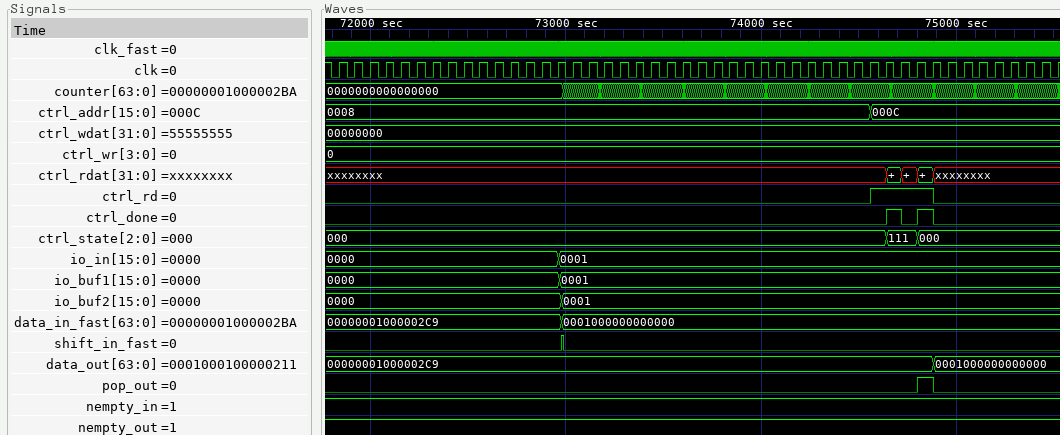
\includegraphics[width=\textwidth]{../figures/simulation_data_in.png}
		\caption[Auszug aus der Simulation des Event-Recorder-Moduls]{Auszug aus der Simulation des Event-Recorder-Moduls}
	\label{fig:ice40_pmod_pins}
\end{figure}

\section{Implementierung eines SPI-Slave-Moduls}
\label{ch:Implementierung:sec:SPI-Slave}

Für den Austausch der Daten mit dem Raspberry Pi wird noch eine weitere Komponente für die SPI-Kommunikation benötigt. Diese Komponente soll wieder als {\tt IcoSoc}-Modul umgesetzt sein, um die Ausführung des C-Codes nicht unnötig zu verlangsamen. Das {\tt IcoSoc}-Projekt enthält bereits ein SPI-Modul, allerdings handelt es sich hier um eine reine Master-Implementierung (vor allem zum Ansprechen externer Hardware wie zum Beispiel kleinerer LCDs). 
Deswegen wurde noch ein zusätzliches SPI-Slave-Modul entworfen.\\
Die Bus-Logik funktioniert analog zum Event-Recorder-Modul, wobei im C-Teil eine ``bidirektionale'' Übertragungsfunktion zur Verfügung gestellt wird. Es wird ein 32-Bit-Wert als Argument übergeben und gleichzeitig einen 32-Bit-Wert als Rückgabe geliefert. 
\begin{minted}{c}
static inline uint32_t icosoc_@name@_xfer(uint32_t value)  
{
    *(volatile uint32_t*)(0x20000004 + @addr@ * 0x10000) = value;
    return *(volatile uint32_t*)(0x20000008 + @addr@ * 0x10000);
}
\end{minted}
Das Argument sind dabei die über SPI zu sendenden Daten, und der Rückgabewert die empfangenen Daten.\\
Der SPI-Transfer ist dabei ähnlich einem Schieberegister implementiert, bei dem bei jeder steigenden Taktflanke ein Bit der Sende-Daten am MISO-Ausgang anliegt, und durch das am MOSI-Eingang anliegende Bit ersetzt wird.
Meist werden dabei nur 8 Bit am Stück übertragen (vgl. \cite{wiki:SPI}), durch die Übertragung von 32-Bit kann im vorliegenden Fall die Übertragungsrate etwas erhöht werden. 

\section{Zusammenführung der Module als Icosoc-Projekt}
\label{ch:Implementierung:sec:Icosoc-Projekt}

\section{Implementierung des textbasierten Benutzerinterfaces}
\label{ch:Implementierung:sec:Benutzerinterface}

\chapter{Anwendungsfall: Jitter-Analyse eines Software-generierten Clock-Signals}
\label{ch:Anwendungsfall}
\ldots

\section{Einrichten des Projekts}
\label{ch:Anwendungsfall:sec:Einrichten}

\ldots


\section{Konfiguration der Event-Trigger}
\label{ch:Anwendungsfall:sec:Event-Trigger}

\ldots
\clearpage


\section{Durchf\"uhren der Event-Aufnahme}
\label{ch:Anwendungsfall:sec:Durchf\"uhrung}

\ldots


\section{Analyse der Ergebnisse}
\label{ch:Anwendungsfall:sec:Analyse}

\ldots



\chapter{Fazit}
\label{ch:Fazit}
%% ==============================
Bla fasel\ldots


\chapter{Aussicht}
\label{ch:Aussicht}
%% ==============================
Bla fasel\ldots








\appendix



%% ++++++++++++++++++++++++++++++++++++++++++
%% Abkürzungsverzeichniss
%% ++++++++++++++++++++++++++++++++++++++++++


%\printglossary[type=\acronymtype] % prints just the list of acronyms
\printglossary[type=\acronymtype,title={Abkürzungen}]
\printglossary[type=main]

%\addcontentsline{toc}{chapter}{\protect\numberline{}{Abk\"urzungsverzeichnis}}
\clearpage

\listoffigures
\addcontentsline{toc}{chapter}{Abbildungsverzeichnis}
\clearpage

\listoftables
\addcontentsline{toc}{chapter}{Tabellenverzeichnis}
\clearpage



\ifnotonesideelse{\cleardoublepage}{}

%% ++++++++++++++++++++++++++++++++++++++++++
%% Literatur
%% ++++++++++++++++++++++++++++++++++++++++++
\addcontentsline{toc}{chapter}{\bibname}
%  mit dem Befehl \nocite werden auch nicht zitierte Referenzen abgedruckt 
% (normalerweise nicht erwünscht)
% \nocite{*}
%\bibliographystyle{plain}
%Einbinden Bibtexdatei - Direkt aus JabRef generiert
%\bibliography{literatur}
\printbibliography 

%%% Anhänge
\chapter{Material}
\label{ch:Material}
\enlargethispage{120cm}
\section{PMOD-Pinbelegung des IceZero-Boards}

Bei der Pin-Belegung wurde das selbe Schema wie beim GPIO-Modul des IcoSoc verwendet. Die Numerierung läuft dementsprechend von rechts nach links und für die einzelnen PMOD-Header ``zeilenweise'' von oben nach unten.

\begin{figure}[h]
	\centering
	\captionsetup{justification=centering,margin=2cm}
		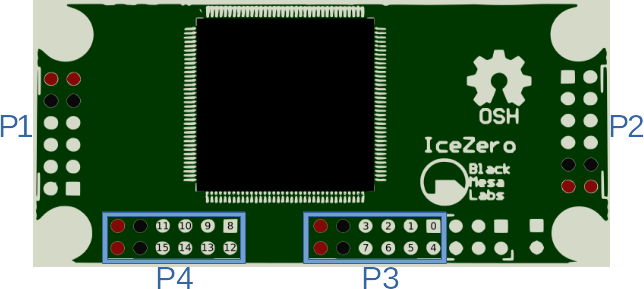
\includegraphics[width=0.80\textwidth]{../figures/ice40_pmod_pins_01.png}
		\caption[Pinbelegung der PMOD-Header des IceZero-Boards]{Pinbelegung der PMOD-Header des IceZero-Boards (Quelle: Eigene Abbildung)}
	\label{fig:ice40_pmod_pins}
\end{figure}

\begin{table}[h]
\centering
\resizebox{\columnwidth}{!}{%
\begin{tabular}{lllllllllllll}
\cline{1-6} \cline{8-13}
\multicolumn{1}{|l|}{\cellcolor[HTML]{DF2727}3.3V} & \multicolumn{1}{l|}{\cellcolor[HTML]{343434}{\color[HTML]{FFFFFF} GND}} & \multicolumn{1}{l|}{pin\_11} & \multicolumn{1}{l|}{pin\_10} & \multicolumn{1}{l|}{pin\_9}  & \multicolumn{1}{l|}{pin\_8}  & \multicolumn{1}{l|}{} & \multicolumn{1}{l|}{\cellcolor[HTML]{DF2727}3.3V} & \multicolumn{1}{l|}{\cellcolor[HTML]{343434}{\color[HTML]{FFFFFF} GND}} & \multicolumn{1}{l|}{pin\_3} & \multicolumn{1}{l|}{pin\_2} & \multicolumn{1}{l|}{pin\_1} & \multicolumn{1}{l|}{pin\_0} \\ \cline{1-6} \cline{8-13} 
\multicolumn{1}{|l|}{\cellcolor[HTML]{DF2727}3.3V} & \multicolumn{1}{l|}{\cellcolor[HTML]{343434}{\color[HTML]{FFFFFF} GND}} & \multicolumn{1}{l|}{pin\_15} & \multicolumn{1}{l|}{pin\_14} & \multicolumn{1}{l|}{pin\_13} & \multicolumn{1}{l|}{pin\_12} & \multicolumn{1}{l|}{} & \multicolumn{1}{l|}{\cellcolor[HTML]{DF2727}3.3V} & \multicolumn{1}{l|}{\cellcolor[HTML]{343434}{\color[HTML]{FFFFFF} GND}} & \multicolumn{1}{l|}{pin\_7} & \multicolumn{1}{l|}{pin\_6} & \multicolumn{1}{l|}{pin\_5} & \multicolumn{1}{l|}{pin\_4} \\ \cline{1-6} \cline{8-13} 
\multicolumn{6}{c}{PMOD - P4}                                                                                                                                                                                                                            &                       & \multicolumn{6}{c}{PMOD - P3}                                                                                                                                                                                                                      
\end{tabular}
}
\caption{Pinbelegung der PMOD-Header des Icezero-Boards}
\label{tbl:PMOD-Pins}
\end{table}


\clearpage
\begin{landscape}

\section{Pinverbindungen Raspberry Pi und FPGA-Shield}

\begin{table}[h]
\centering
\caption{Pinbelegung}
\label{tbl:Pinbelegung}
\begin{tabular}{|l|l|l|
>{\columncolor[HTML]{EFEFEF}}l |
>{\columncolor[HTML]{EFEFEF}}l |l|l|l|}
\hline
\cellcolor[HTML]{C0C0C0}ice40 & \cellcolor[HTML]{C0C0C0}WiringP & \cellcolor[HTML]{C0C0C0}Name                       & \multicolumn{2}{l|}{\cellcolor[HTML]{C0C0C0}Physical} & \cellcolor[HTML]{C0C0C0}Name                       & \cellcolor[HTML]{C0C0C0}WiringPi & \cellcolor[HTML]{C0C0C0}ice40 \\ \hline
                              &                                 & \cellcolor[HTML]{DF2727}3.3V                       & 1                         & 2                         & \cellcolor[HTML]{DF2727}5V                         &                                  &                               \\ \hline
                              & 8                               & SDA.1                                              & 3                         & 4                         & \cellcolor[HTML]{DF2727}5V                         &                                  &                               \\ \hline
                              & 9                               & SCL.1                                              & 5                         & 6                         & \cellcolor[HTML]{000000}{\color[HTML]{FFFFFF} GND} &                                  &                               \\ \hline
                              & 7                               & 1-Wire                                             & 7                         & 8                         & TxD                                                & 15                               &                               \\ \hline
                              &                                 & \cellcolor[HTML]{000000}{\color[HTML]{FFFFFF} GND} & 9                         & 10                        & RxD                                                & 16                               &                               \\ \hline
                              & 0                               & GPIO. 0                                            & 11                        & 12                        & GPIO.1                                             & 1                                &                               \\ \hline
                              & 2                               & GPIO. 2                                            & 13                        & 14                        & \cellcolor[HTML]{000000}{\color[HTML]{FFFFFF} GND} &                                  &                               \\ \hline
                              & 3                               & GPIO. 3                                            & 15                        & 16                        & GPIO. 4                                            & 4                                &                               \\ \hline
                              &                                 & \cellcolor[HTML]{DF2727}3.3V                       & 17                        & 18                        & GPIO. 5                                            & 5                                &                               \\ \hline
                              & 12                              & MOSI                                               & 19                        & 20                        & \cellcolor[HTML]{000000}{\color[HTML]{FFFFFF} GND} &                                  &                               \\ \hline
                              & 13                              & MISO                                               & 21                        & 22                        & GPIO. 6                                            & 6                                &                               \\ \hline
                              & 14                              & SCLK                                               & 23                        & 24                        & CE0                                                & 10                               &                               \\ \hline
                              &                                 & \cellcolor[HTML]{000000}{\color[HTML]{FFFFFF} GND} & 25                        & 26                        & CE1                                                & 11                               &                               \\ \hline
                              & 30                              & SDA.0                                              & 27                        & 28                        & SCL.0                                              & 31                               &                               \\ \hline
			      & 21                              & GPIO.21                                            & 29                        & 30                        & \cellcolor[HTML]{000000}{\color[HTML]{FFFFFF} GND} &                                &                               \\ \hline
                              & 22                              & GPIO.22                                            & 31                        & 32                        & GPIO.26                                            & 26                               &                               \\ \hline
                              & 23                              & GPIO.23                                            & 33                        & 34                        & \cellcolor[HTML]{000000}{\color[HTML]{FFFFFF} GND} &                                &                               \\ \hline
                              & 24                              & GPIO.24                                            & 35                        & 36                        & GPIO.27                                            & 27                               &                               \\ \hline
                              & 25                              & GPIO.25                                            & 37                        & 38                        & GPIO.28                                            & 28                               &                               \\ \hline
                              &                                 & \cellcolor[HTML]{000000}{\color[HTML]{FFFFFF} GND} & 39                        & 40                        & GPIO.29                                            & 29                               &                               \\ \hline
\end{tabular}
\end{table}
\end{landscape}

\clearpage

\section{CD}
Die beiliegende CD enthält den Inhalt des Github-Repositories 
\begin{lstlisting}[language=bash]
https://github.com/dm7h/fpga-event-recorder
\end{lstlisting}
zum Zeitpunkt der Abgabe.

Folgende Tabelle entält einen Überblick über die Inhalte des Repositories:
\begin{table}[h]
\centering

\begin{tabular}{|p{1cm}|p{3cm}|p{10cm}|}
\hline
\rowcolor[HTML]{C0C0C0} 
Verz. & Unterverzeichnis                & Inhaltsbeschreibung                                                                                                                                                                                                                                                                                                      \\ \hline
doc/        & ref/                            & iCE40 Manuals und relevante Hardwaredokumentation                                                                                                                                                                                                                                                                        \\ \hline
thesis/     &                                 & Finale Version der Bachelorarbeit als PDF                                                                                                                                                                                                                                                             \\ \hline
thesis/     & src/                            & Latex-Sourcen der Bachelorarbeit                                                                                                                                                                                                                                                              \\ \hline
src/        &                                 &                                                                                                                                                                                                                                                                                                                          \\ \hline
            & Logikanalysator/                & Dateien des Semesterprojekts ``Logikanalysator mit AVR Mega32U4 und Altera MAX CPLD''  inkl. Dateien der Bachelorarbeit von Andreas Müller (USB-TPLE)  
															     \\ \hline
            & icotools/                       & Portierung des icotools Projekts für das IceZero-Board. Original-Repository: https://github.com/cliffordwolf/icotools. Relevant sind hier vor allem die Unterverzeichnisse ``icosoc'' und ``icoprog'' 
\\ \hline
            & icozctl/                        & Fork des icoprog-Tools (icotools/icoporg) mit zusätzlichen Funktionen zur Steuerung des Event-Recorders                                                                                                                                                                                                                  \\ \hline
            & icozero/                        & Vom IcoSoc unabhängiges Beispiel-Projekt für das IceZero-Board mit leichten Modifikationen (nicht projekt-relevant)                                                                                                                                                                                                      \\ \hline
            & picosoc/                        & Portierung des PicoSoc-Projekts auf das IceZero-Board (nicht direkt projekt-relevant). PicoSoc ist eine minimale Variante des IcoSocs. Original-Repository: https://github.com/cliffordwolf/picorv32/tree/master/picosoc                                                    \\ \hline
            & sump2/                          & SUMP2 Variante für das IceZero-Board (nicht für die Icestorm-Toolchain)                                                                                                                                                                                                                                                  \\ \hline
            & sump2\_pipistrello\_ ftdi\_fifo/ & SUMP2 Vairante für das Pipistrello-Board bei dem der Versuch unternommen wurde den UART durch einen FTDI-Fifo zu ersetzen, um einen Höheren Datenduchsatz zu ermöglichen. Quelle: http://forum.gadgetfactory.net/topic/1748-open-bench-logic-sniffer-with-64mb-capture-buffer/ \\ \hline
            & demon-core-import/              & SUMP2 Weiterenwicklung für den Open Bench Logic Sniffer. Quelle: https://github.com/jhol/demon-core-import                                                                                                                                                                     \\ \hline
\end{tabular}
\caption{Überblick über den Inhalt des Git-Repositories}
\label{tbl:git_repo}
\end{table}

\chapter{GPL}
\label{ch:GPL}
%% ==============================
Anhang B \ldots




%% ++++++++++++++++++++++++++++++++++++++++++
%% Index (optional)
%% ++++++++++++++++++++++++++++++++++++++++++
%\ifnotdraft{
\addcontentsline{toc}{chapter}{Index}
\printindex            % Index, Stichwortverzeichnis
%}

\clearpage
\chapter*{Erklärung zum Abschlussbericht}
Hiermit versichere ich, die eingereichte Abschlussarbeit selbständig verfasst und keine andere als die von mir angegebenen Quellen und Hilfsmittel benutzt zu haben. Wörtlich oder inhaltlich verwendete Quellen wurden entsprechend den anerkannten Regeln wissenschaftlichen Arbeitens zitiert. Ich erkläre weiterhin, dass die vorliegende Arbeit noch nicht anderweitig als Abschlussarbeit eingereicht wurde. Das Merkblatt zum Täuschungsverbot im Prüfungsverfahren der Hochschule Augsburg habe ich gelesen und zur Kenntnis genommen. Ich versichere, dass die von mir abgegebene Arbeit keinerlei Plagiate, Texte oder Bilder umfasst, die durch von mir beauftragte Dritte erstellt wurden.

\vspace{4cm}

\hspace{2cm} Ort, Datum \hfill Unterschrift \hspace{2cm}


\end{document}
